\section{Produktudformning}
\subsection{Overordnet}
Koden er opbygget, således at den kan skrives som en pseudo-webapplikation, sidenhen anvendes en "bro", der gør til en native applikation og kompatibel med de mest almindelige styresystemer, herunder IOS (Apples mobile styresystem) og Android\footnote{Selvsamme teknik anvendes af højtprofilerede virksomheder, såsom Facebook, Discord og Tesla. Læs mere her: \href{https://reactnative.dev/}{reactnative.dev}}.

\subsection{Kodestack}
\subsubsection{Framework - React Native \label{sec:reactnative}}
React Native er et framework\footnote{Et >>framework<< er en samling af biblioteker, der gør det lettere at skrive kode på en standardiseret måde, hvori en masse valg er taget på forhånd}, der muliggør udvikling af native\footnote{>>Native<< betyder at applikationen kører direkte på den pågældende enhed} applikationer til IOS og Android. 
\subsubsection{Sub-Framework - Expo}
Expo er et framework, der er bygget omkring React Native, der muliggør at køre en pågældende React Native-applikation igennem deres egen platform, Expo Go, hvorfor er smart, fordi man ikke behøver at kompile koden, dvs. oversætte programmeringskoden til eksekverbar maskinekode, efter hver ændring, såfremt man vil teste den på en fysisk enhed. 
\subsubsection{Runtime - Node.js}
Node.js er den runtime, der muliggør, at applikationen kan køre på en enhed fremfor i en browser, da programmeringssproget JavaScript oprindeligt var designet til at køre udelukkende i et browser-miljø. Dette er altså en nødvendighed for, at applikationen skal kunne køre på en fysisk enhed.
\subsubsection{Database - MongoDB*}
Ideen var oprindeligt at have en meget let applikation, der kunne nedhentes fra et styresystems nativ app-bibliotek, hvorefter denne ville prompte brugeren til at nedhente ekstrapakker, fx videoer og manualer, fra vores egen server, som skulle være administreret via MongoDB. MongoDB er et program, som tillader en at lave og administrere en NoSQL-database, i stedet for en SQL-database, da det er mere skalerbart og fleksibelt i den forstand, at man hurtigt kan tilføje nye data, fx brødtekst, og hente disse. 
\subsubsection{Programmeringsprog - Typescript}
Typescript er et programmeringssprog udviklet af Microsoft, som bygger på JavaScript. Typescipt bruger stærke datatyper, hvilket vil sige, at datatypen angives per data. Typescript anvendes i denne applikation, fordi det er et kompilersprog, hvilket vil sige, at fejl kan blive fanget, når koden kompileres, fremfor i runtime, mens programmet kører, hvilket er en stor fordel i programmeringsprocessen, da det hindrer, at der kommer oversete fejl i koden.
\subsection{Brugergrænseflade}
Brugergrænsefladen er det, brugeren oplever, når han interagerer med applikationen. Brugergrænsefladen er blevet tegnet i Figma, et program, som er speciallavet til at konstruere brugergrænseflader, bl.a. har den prælavede elementer, fx knapper og tekstinputfelter, desuden kan dette gøres interaktivt. 
\subsubsection{Konceptdesign}
Jf. appendiks \ref{apx:konceptart} er følgende skitser blevet udarbejdet. Herefter er disse blevet implementeret i selve applikationen. Brugergrænseflade består primært af en bjælke, der er placeret i bunden af skærmen, hvorfra brugeren kan navigere mellem forskellige sider.
\subsubsection{Design}

\subsection{Produktgennemgang}
Koden samt ideerne som applikationen bygger på, vil blive gennemgået nedenfor.
\subsubsection{Filstruktur}

Måden hvorpå filerne er struktureret, er altafgørende for kodens funktionalitet og læsbarhed. Da frameworket React Native, kigger efter spicifikke filstrukturer, til at køre og vise den dertilhørende kode det korrekte sted.
\begin{figure}[H]
    \dirtree{%
        .1 /.
        .2 {\color{blue}{app}}.
        .2 {\color{blue}{assets}}.
        .2 {\color{blue}{components}}.
        .2 {\color{blue}{constants}}.
        .2 {\color{blue}{data}}.
        .2 {\color{blue}{hooks}}.
        .2 {\color{blue}{node\_modules}}.
        .2 {\color{blue}{scripts}}.
        .2 .gitignore.
        .2 app.json.
        .2 babel.config.js.
        .2 eas.json.
        .2 package-lock.json.
        .2 package.json.
        .2 tsconfig.json.
       }
    \caption{Top-level filstrukturen for applikationen. Mapperne er farvet blåt}
    \label{fig:tlprojstruct}
\end{figure}

Måden, hvorpå brugeren navigerer applikationen, er ved at bruge en navigationsbar, som er placeret i bunden af skærmen. 
Filstrukturen som viser navigationsbaren, ser således ud i kodebasen:
\begin{figure}[H]
    \dirtree{%
        .1 /app.
        .2 {\color{blue}{(tabs)}}.
        .3 {\color{blue}{afgrøde-beregner}}.
        .3 {\color{blue}{bibliotek}}.
        .3 {\color{blue}{e-beregner}}.
        .3 {\color{blue}{indstillinger}}.
        .3 \_layout.tsx.
        .3 index.tsx.
        .2 \_layout.tsx.
        .2 +not-found.tsx.
       }    
    \caption{Top-level filstrukturen for routes-systemet. Mapperne er farvet blåt}
    \label{fig:tlprojstruct}
\end{figure}

Det smarte ved netop denne filstruktur, er at det er komponentbaseret, hvilket vil sige, at man kan hente og genbruge komponenter fra mappen med disse, hvorfor koden bliver mere effektiv, da man ikke behøver genkode tidligere kodede elementer. 

\subsubsection{Bibliotekskoden}
Her benytes dynamic-routes\footnote{>>Dynamic routes<< er en funktion i React-frameworket \ref{sec:reactnative}, som gør man kan lave routes ud fra dynamisk data. Man kan forestille sig fx en generisk side, der populeres med data hentet eksternt, fx dens rubrik, underrubrik, url, etc.} til at hente brødtekst og rubrikker fra en database. Dette muliggør, at navigationsbjælken til højre kan være renderet konstant, mens den til højre (se nedenfor illustration) kan være renderet dynamisk, alt efter hvilken route brugeren befinder sig på. Læg mærke til, at det er opdelt via en flexboks\footnote{>>Flexbox<< er en form for gitter, der skaleres dynamisk ift. de omkringliggende elementer.}, hvilket gør, at der er fire kasser, de to yderste til venstre indeholder kun tekst, hvor de to til højre kan indeholde tekst, billeder og videoer, som hver især optager 50\% af den resterende (navigationsbjælken optager også plads) skærmplads.

\begin{figure}[H]
    \centering
    \fbox{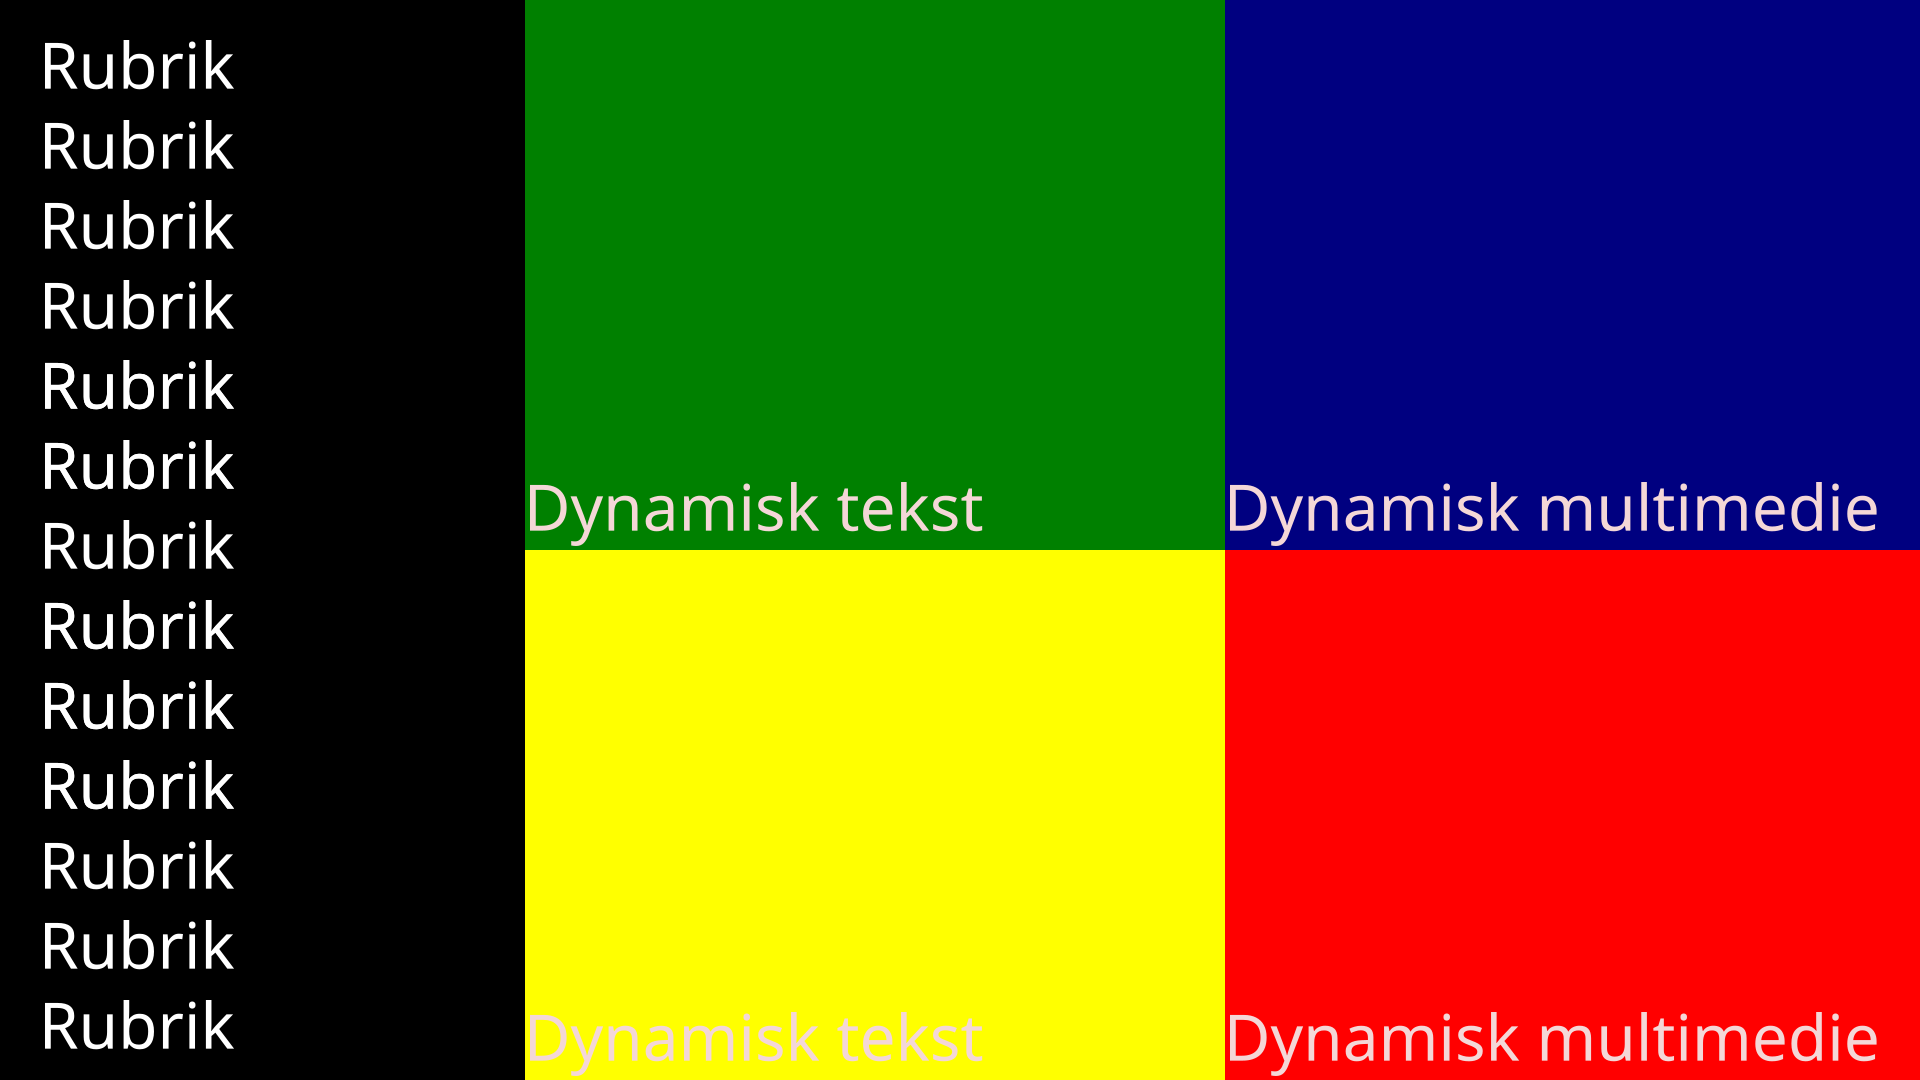
\includegraphics[width=\textwidth]{assets/section_6/Illustration-dynamic-routes.png}}
    \caption{Illustration af routes-systemet}
    \label{fig:routes}
\end{figure}

I det her tilfælde, laves datakald til en JSON-fil\footnote{JSON (JavaScript Object Notation) filer er et letvægts- læsbart filformat, som bruges til at organisere / strukturere information}. Denne svarer i samme format, som en database ville, hvorfor dette er anvendt til at demonstrere datahåndteringsfunktionalitet uden at en reel database er nødvendig. I kapitlet \ref{sec:produktionsforberedelse} kan der læses mere om en eventuel implementering af en database.

\subsubsection{E-beregner}
E-beregneren er en simpel beregner, der har til formål at informere brugeren om, hvor stort deres kalorieindstag skal være ud fra nogle data. Denne tager højde for BMR, basalmetabolisme, som udgør ca 70\% af totalenergiforbruget og PA, fysisk aktivitet, som udgør ca. 20\% men ikke DIT, diætinduceret varmedannelse, som udgør 10\%\cite{EE-artikel}.

\paragraph{Matematikken}
Til formålet anvendes basalmetabolisme, som beskriver et varmblodet dyrs stofskifte.\cite{BMR-artikel} Her tages udgangspunkt i menneskets basalmetabolisme. Til dette formål anvendes Harris-Benedict-formlen, som er blevet revideret af Mifflin og St. Jeor i 1990\cite{Harris-Benedict-formel}, der ser således ud:

For mænd:
\begin{equation}
    \text{BMR} \left[\dfrac{\text{kcal}}{\text{dag}}\right] = (10 \cdot \text{vægt [kg]}) + (6,25 \cdot \text{højde [cm]}) - (5 \cdot \text{alder [år]}) + 5
\end{equation}

For kvinder:
\begin{equation}
    \text{BMR} \left[\dfrac{\text{kcal}}{\text{dag}}\right] = (10 \cdot \text{vægt [kg]}) + (6,25 \cdot \text{højde [cm]}) - (5 \cdot \text{alder [år]}) - 161
\end{equation}

Forskellen i formlen, skyldes mænd har en lidt højere basalmetabolisme end kvinder.

For at estimere det resterende kalorieforbrug, multipliceres BMR med en konstant, som afhænger af en persons fysiske aktivitet. Tallene er fundet fra en beregner på nettet med lignende funktionalitet \cite{OMNI-calc}:
\begin{table}[H]
    \centering
    \begin{tabular}{|c|c|}
        \hline
        \textbf{Aktivitet} & \textbf{Konstant} \\
        \hline
        Sedentær & 1,2 \\
        Lidt eller ingen aktivitet & 1,4 \\
        Let aktivitet 1-2 gange om ugen & 1,6 \\
        Moderat Aktivitet 2-3 gange om ugen & 1,75 \\
        Hård aktivitet 3-5 gange om ugen & 2 \\
        Fysisk job eller hård daglig aktivitet & 2,4 \\
        \hline
    \end{tabular}
\end{table}

Herefter skal der tages højde for, om brugeren er fysisk aktiv, hvilket vil sige, at der skal ganges med en faktor, der er 1,2 for personer, der er særdeles fysisk aktive, til 1,9 for personer, der er ekstremt fysisk aktive.
\paragraph{Implementering heraf}